\section{Forschungsmethode}
\label{sec:Forschungsmethode}
Den Richtlinien in \cite{Keele2007GuidelinesEngineering} folgend, wurde ein Systematisches Literatur Review (SLR) nach Kitchenham et al. durchgeführt. Das Dokument folgt dem Aufbau in \cite{Walia2009AErrors} und umfasst die folgenden Schritte 

\begin{itemize}
    \item Formulierung eines Review-Protokolls
    \item Durchführen des Reviews
        \begin{itemize}
            \item Identifizierung von Primärstudien
            \item Evaluierung \& Auswahl
            \item Datenextraktion
            \item Datensynthese
        \end{itemize}
    \item Analyse der Ergebnisse
    \item Auswertung der Ergebnisse
    \item Diskussion der Ergebnisse
\end{itemize}

Ein Review Protokoll enthält alle Forschungsfragen, Methoden, Vorgehensweisen etc. die benötigt werden um ein SLR durchführen zu können Es wird im Vorfeld des Reviews angefertigt, um zu vermeiden, dass das Review durch die Erwartungshaltung des Forschers getrieben wird und damit an Objektivität verliert (Reseracher bias). Nach Durchführung des Reviews wird aus den Ergebnissen der Datensynthese eine Analyse und Auswertung der Ergebnisse durchgeführt um die gestellten Forschungsfragen beantworten zu können \cite{Walia2009AErrors}.

\subsection{Forschungsfragen}

Das zentrale Ziel dieses SLR war es, Qualitätsprobleme im Management der Requirements Traceability und mögliche Lösungsanasätze zu identifizieren und zu klassifizieren. Die zugehörige Fragestellung für den Review war also

\enquote{Welche Arten von Qualitätsprobleme existieren im Management der Requiremenst Traceability und wie können diese behoben werden?}

Zur Beantwortung der Fragestellung, war es notwendig entsprechende Forschungsfragen zu definieren, die sich auf die Beantwortung dieser Fragestellung fokussierten und damit im Review auch zu verwertbaren Ergebnissen führten. Nach einer ersten Analyse des Forschungsgebietes, konnte festgestellt werden, dass ein Teil der Forschungsarbeiten sich nur indirekt auf Qualitätsprobleme im Management von Requirements Traceability bezogen. Im Fall, dass ein Lösungsansatz zur Thematik genannt worden ist, war dieser nicht zwingend nur für den speziellen Anwendungsfall einsetzbar.

Aus den Ergebnissen der Analyse konnte eine Vorgehensweise identifiziert werden, die die Beobachtungen wiederspiegelte und im Einklang mit dem Forschungsfrage dieses Reviews stand. Die Abbildung \ref{fig:abb_forschungsfragen} zeigt das Ergebnis der ersten Analysephase und damit die Festlegung der Vorgehensweise für den weiteren Reviewverlauf

\begin{figure}[!htb]
  \centering
  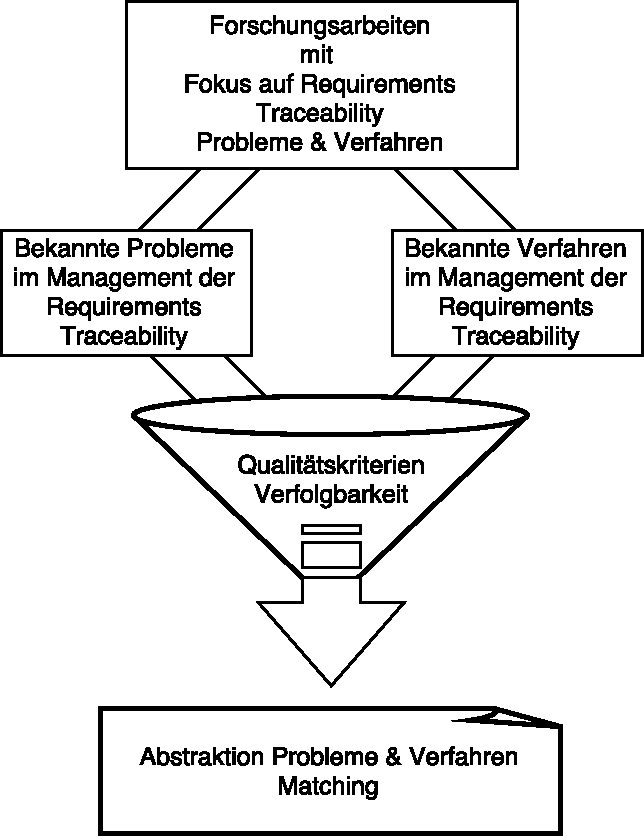
\includegraphics[width=2in]{forschungsfragen_diagramm_v2.pdf}
  \caption{Vorgehensweise zur Beantwortung der Forschungsfragen}
  \label{fig:abb_forschungsfragen}
\end{figure}

% Ggf. anhand des Forschungsziels nochmal zu präzisieren!
Wie in \ref{fig:abb_forschungsfragen} dargestellt wurde das Vorgehen in mehrere Etappen eingeteilt. Im ersten Schritt stand die Identifikation von Forschungsarbeiten die im Themengebiet Requirements Traceability angesiedelt waren und sich mit Problemen oder Lösungsansätzen in diesem Bereich beschäftigten. Entsprechend mussten die Forschungsfragen und Auswahlkriterien so formuliert werden, dass die entsprechenden Arbeiten erfasst wurden. Anhand der Analyse wurde sich dazu entschieden, im weiteren Verlauf Probleme und Verfahren zu separieren und in Bezug zu den Qualitätskriterien zu stellen, da nach den Ergebnissen aus der Analyse nicht jeder Lösungsansatz auf einen Anwendungsfall beschränkt war. Im letzten Schritt folgte dann eine Zusammenführung aller Daten um die Abdeckung von Problemen und Verfahren zu bestimmen um die zentrale Forschungsfrage beantworten zu können.

Die Tabelle \ref{tab:forschungsfragen} zeigt die Forschungsfragen, die aus der Vorgehensweise und der zentralen Fragestellung für diesen Review extrahiert wurden. Um Willkür zu vermeiden, wurde in Tabelle \ref{tab:motivationen} zu jeder Frage eine Motivation niedergeschrieben, die die Sinnhaftigkeit einer Frage separat darstellt. Die erste Frage befasst sich mit möglichen Qualitätsproblemen im Management der Requirements Traceability mit dem Ziel, diese möglichst vollständig zu erfassen. Die zweite Frage befasst sich separat mit den Verfahren zu Behandlung von Qualitätsproblemen und Hinweisen dazu in den erfassten Forschungsarbeiten. Die dritte und letzte Frage fasst die gesammelten Daten zu abstrakteren Vorgehensweisen zusammen, anhand derer ein Abdeckungsgrad für klassifizierte Qualitätsprobleme bestimmt werden kann. Die Fragen 1 und 2 erforderten einen systematische Literaturreview.

% ------------------------------------------------------------------------------------------
% --- FORSCHUNGSFRAGEN + MOTIVATIONE

\begin{table*}[t]
\renewcommand{\arraystretch}{1.3}
\centering
\begin{tabularx}{\textwidth}{@{}X@{}}
\toprule
Forschungsfragen \\ \midrule
1. Welche Arten von Qualitätsproblemen können während des Softwarelebenszyklus im Management der Requirements Traceability entstehen? \\
\hspace*{10mm}1.1 Welche Arten von Qualitätsproblemen in der Requirements Traceability wurden in der vorhandenen Literatur identifiziert? \\
\hspace*{10mm}1.2 Welche Qualitätsprobleme können durch die Analyse ihrer Ursache identifiziert werden? \\
\hspace*{10mm}1.3 Beeinflussen die gefundenen Probleme die Kriterien in \ref{tab:qualitaet_verfolgbarkeit}? \\
2. Welche Verfahren existieren im Management der Requirements Traceability zur Behandlung von Qualitätsproblemen? \\
\hspace*{10mm}2.1 Greift die Literatur Prozesse oder Methodiken auf, die zu einer Verbesserung der Qualität beitragen? \\
\hspace*{10mm}2.2 Addressieren die gefundenen Verfahren die Kriterien in \ref{tab:qualitaet_verfolgbarkeit}? \\
3. Lassen sich die Erkenntnisse aus 1-2 zu Aussagen über mögliche Verfahrensweisen im spezifischen Anwendungsfall zusammenfassen? \\
\bottomrule
\end{tabularx}
\caption{Definierte Forschungsfragen}
\label{tab:forschungsfragen}
\end{table*}

\begin{table*}[t]
    \centering
    \begin{tabularx}{\textwidth}{X}
        \toprule
        Motivationen \\ \midrule
        1. Unabhängige Erfassung aller Qualitätsprobleme die mindestens eine der Kriterien für Qualität von Verfolgbarkeit beinflussen \\
        2. Unabhängige Erfassung aller Verfahren die mindestens einer der Kriterien für Qualität von Verfolgbarkeit beeinflussen \\
        3. Bestimmen von Verfahren und ihrer Abdeckung für die Behandlung von Qualitätsproblemen \\
    \bottomrule
    \end{tabularx}
    \caption{Motivationen zu den gestellten Forschungsfragen in \ref{tab:forschungsfragen}}
    \label{tab:motivationen}
\end{table*}

% ------------------------------------------------------------------------------------------

\subsection{Quellenauswahl und Suche}
\label{subsec:Quellenauswahl}

Die initiale Auswahl der Quellen erfolgte anhand der unten beschriebenen Auswahlkriterien:

\begin{itemize}
    \item Es wurde nach Datenbanken gesucht, die:
        \begin{itemize}
            \item Veröffentlichungen aus Zeitschriften oder Konferenzen über Software Engineering oder Software Qualität enthielten
            \item Eine Suchmaschine mit erweitertem Suchmechanismus offerierten. Der Suchmechanismus musste die Expertensuche nach einer Folge von logischen Ausdrücken unterstützen
            \item Das Volltextdokument musste über die Datenbank oder andere Hilfsmittel abrufbar sein
        \end{itemize}
    \item Die gefundenen Datenbanken wurden auf ein minimales Set reduziert um die Anzahl redundanter Papiere minimal zu halten
    \item Andere Quellen wurden hinzugefügt, die nach Einschätzung des Forschers eine relevanz zum Thema haben
\end{itemize}

Eine Einschränkung der Datenbanken auf Zeitschriften und Konferenzen im Bereich Software Engineering oder Software Qualität ergab sich aus der initialen Analyse unter der Berücksichtigung, das dass Management der Requirements Traceability teil des Requirements Engineering im Software Engineering ist. Da der Fokus dieser Arbeit auf Qualität lag, wurde sich letztendlich für die oben genannten Bereiche entschieden um den Suchraum möglichst weit zu fassen. Der erweiterte Suchmechanismus nach logischen Ausdrücken war Vorraussetzung für die geplante Suche nach Suchstrings auf die in diesem Kapitel noch näher eingangen wird. Neben den klassischen Datenbanken war es nach der Auffassung des Forschers notwendig, weitere Quellen wie Buchquellen zu betrachten um die Vollständigkeit des Reviews sicherzustellen. Da Forschungspapiere in mehreren Datenbanken auftauchen konnten und dies einen erheblichen Mehraufwand bedeutet hätte, wurden die gefundenen Datenbanken auf ein minimales Set reduziert um die Anzahl redundanter Papiere zu minimieren. Tabelle \ref{tab:quellen_review} zeigt das Ergebnis der Quellenauswahl

\begin{table}[!ht]
\renewcommand{\arraystretch}{1.3}
\centering
\begin{threeparttable}
\begin{tabularx}{\columnwidth}{@{}lX@{}}
\toprule
Kriterium & Auswirkung\\ \midrule
Datenbanken & ACM Digital Library, IEEE Xplore, Science Direct (Elsevier), SpringerLink\\
Andere Artikel & SWEBOK - Software Engineering Body of Knowlege\\
Erweiterte Quellen & Buchquellen \\
\bottomrule
\end{tabularx}
\medskip
      %\footnotesize\textbf{Legende:}\smallskip
      %\begin{tablenotes}\footnotesize
      %\item[*] In \cite{Kollanus2010Test-DrivenApproach} werden die gleichen Studien wie in \cite{Kollanus2011CriticalDevelopment} untersucht.
      %\end{tablenotes}
\end{threeparttable}
\caption{Quellen für den Review}
\label{tab:quellen_review}
\end{table}

Um die Datenbanken zu durchsuchen, wurden aus den zu reviewenden Forschungsfragen 1-2 übergeordnete Suchbegriffe in englischer Sprache abgeleitet. Diese wurden dann mit Synonymen, Abkürzungen und alternativen Schreibweisen aus den in der Analyse gefundenen Büchern, Papieren etc. angereichtert um eine weite Abdeckung des Suchbegriffes sicherzustellen. Da aus der Analyse hervorging, dass Lösungsansätze und Probleme üblicherweise im selben Dokument genannt werden, wurde sich für die Konstruktion eines globalen Suchstrings entschieden, dessen Ergebnisse dann für den Review beider Forschungsfragen verwendet worden ist. Im folgenden der globale Suchstring der für die Suche in den Datenbanken verwendet worden ist

\enquote{((requirements traceability OR traceability) AND (quality OR condition OR character OR property OR attribute OR aspect) AND (problem OR error OR mistake OR reason OR fault OR defect OR inconsistent OR incomplete OR flaw OR lapse OR slip OR err) AND ((abstraction OR root cause OR cause OR origin OR element OR source) OR (improvement OR method OR technique OR approach OR mechanism OR process OR taxonomy) OR (identify OR analyze OR classify) OR (recovery OR reconstruction OR restoration OR recall) OR (correction OR adjustment OR improvement OR amelioration)))}

Wenn sinnvoll wurden die Filterkriterien dem Fokus des Reviews angepasst und in der Durchführung dokumentiert. Die Auswahl der gefundenen Papiere erfolgte dann in einem mehrstufigen Selektionsprozess. Er umfasste die folgenden Schritte

\begin{enumerate}
    \item Lesen des Titels um Papiere auszuschließen, die keinen klaren Bezug zum Thema haben
    \item Lesen des Abstracts um Papiere weiter anhand ihres Bezugs zum Thema einzugrenzen
    \item Prüfen der Papiere auf die definierten Inklusions- und Exklusionskriterien in \ref{tab:inklusions_exklusionkriterien} um den Bezug zum Thema klar herauszustellen
    \item Prüfen der Papiere auf die definierten Qualitätskriterien in Tabelle \ref{tab:qualitaetskriterien_review} um die Qualität der Forschungsarbeit sicherzustellen
\end{enumerate}

Bei der Durchführung des Reviews musste eine zusätzliche Rahmenbedingung neben dem Selektionsprozess eingeführt werden. Beim Durchsuchen der ersten Datenbank "Science Direct (Elsevier)" wurde das Limit der Anzeige von Suchergebnisse erreicht (1000). Beim Review der bisher gesammelten Treffer konnte zudem festgestellt werden, dass die Trefferquote nach den ersten Seiten dramatisch sank. Daher wurde auf Grund der Limitierung, der durchschnittlichen Anzahl an Treffer pro Datenbank (> 2000) sowie der stark sinkenden Trefferquote das Limit für die Suche in einer Datenbank auf die ersten 10 Ergebnisseiten limitiert.

Für den Review galt es noch die Inklusions- und Exklusionskriterien, sowie Qualitätskriterien für die finale Auswahl von Forschungspapieren zu definieren. Tabelle \ref{tab:inklusions_exklusionkriterien} zeigt die Inklusions- und Exklusionkriterien wie sie für den Review angewendet wurden.

\begin{table}[!ht]
\renewcommand{\arraystretch}{1.3}
\centering
\begin{threeparttable}
\begin{tabularx}{\columnwidth}{@{}XX@{}}
\toprule
Inklusionskriterien & Exklusionskriterien \\ \midrule
Forschungsarbeit beschäftigt sich mit Problemen in der Requirements Traceability & Forschungsarbeit hat keinen Bezug zum Forschungsgebiet \\
Forschungsarbeit beschäftigt sich mit Ursachen für Problemen in der Requirements Traceability & Forschungsarbeit hat keinen Bezug zu den gestellten Forschungsfragen \\
Forschungsarbeit beschäftigt sich mit Methodiken im Management der Requirements Traceability & Forschungsarbeit ist nicht auf Englisch \\
Empirische Studie (qualitative und quantitative) über Praktiken im Management von Requirements Traceability & Ergebnisse einer Forschungsarbeit sind unklar oder mehrdeutig \\
\bottomrule
\end{tabularx}
\medskip
      %\footnotesize\textbf{Legende:}\smallskip
      %\begin{tablenotes}\footnotesize
      %\item[*] In \cite{Kollanus2010Test-DrivenApproach} werden die gleichen Studien wie in \cite{Kollanus2011CriticalDevelopment} untersucht.
      %\end{tablenotes}
\end{threeparttable}
\caption{Inklusions- und Exklusionkriterien}
\label{tab:inklusions_exklusionkriterien}
\end{table}

Die Inklusionskriterien wurden so gewählt, dass sie den Themenbezug zur Requirements Traceability und den Forschungsfragen herausstellten. Die Exklusionskriterien grenzten dies weiter ab. Zusätzlich wurden direkte Ausschlusskriterien eingefügt ohne die eine Forschungsarbeit nicht verwertbar gewesen wäre. Als letzte Instanz für die Auswahl standen die Qualitätskriterien in Tabelle \ref{tab:qualitaetskriterien_review}.

\begin{table}[!ht]
\renewcommand{\arraystretch}{1.3}
\centering
\begin{threeparttable}
\begin{tabularx}{\columnwidth}{@{}XX@{}}
\toprule
Qualitätskriterien \\ \midrule
Basiert die Studie auf sinnvollen Annahmen? \\
Ist die Vorgehensweise angemessen? \\
Werden in der Studie Maßnahmen angewendet, um Mehrdeutigkeiten zu vermeiden? \\
Kann die Studie nachvollzogen werden? \\
\bottomrule
\end{tabularx}
\medskip
      %\footnotesize\textbf{Legende:}\smallskip
      %\begin{tablenotes}\footnotesize
      %\item[*] In \cite{Kollanus2010Test-DrivenApproach} werden die gleichen Studien wie in \cite{Kollanus2011CriticalDevelopment} untersucht.
      %\end{tablenotes}
\end{threeparttable}
\caption{Qualitätskriterien}
\label{tab:qualitaetskriterien_review}
\end{table}

Ihre Aufgabe bestand in der Qualitätssicherung um nur Forschungsarbeiten in die finale Liste aufzunehmen, die den Mindestanforderungen an die Qualität genügten.

\subsection{Durchführung}

Von den 4 identifizierten Datenbanken konnten nur 3 durchsucht werden, da die IEEXplore Datenbank zwar den Kriterien für die Auswahl von Datenbanken entsprach, aber ein Limit von 15 Schlüsselwörtern für logische Ausdrücke hatte. Die Anwendung des globalen Suchstrings war daher nicht möglich. 

Die Suche in den verbleibenden 3 Datenbanken ergab über 10000 Treffer wobei 60\% davon in der ACM Digital Library gefunden wurden. Den festgelegten Rahmenbedingungen im Selektionsprozess folgend, wurden nur jeweils die ersten 10 Ergebnisseiten anhand der Selektionskriterien bewertet. Insgesamt sind 650 Papiere bewertet worden, davon wurden 92 anhand ihres Titels ausgewählt. Nach Lesen des Abstracts blieben noch 35 Forschungsarbeiten übrig, von denen 14 nach Lesen des Volltextes den festgelegten Inklusions- und Exklusionskriterien genügten. Erfreulicherweise waren alle ausgewählten Forschungsarbeiten von hoher Qualität und entsprachen den Qualitätskriterien.

In Tabelle \ref{tab:quellenauswahl_quote} sind die Ergebnisse des Reviews nochmal aufgesplittet. Anhand der Ergebnisse kann festgehalten werden, das die initiale Trefferquote mit \~15\% über den Erwartungen lag und obwohl in der Datenbank ScienceDirect 50 Forschungsarbeiten mehr durchsucht wurden, die Quote nur marginal höher war. Das ist ein gutes Indiz für die Korrektheit der Annahme das die Trefferquote in späteren Ergebnisseiten signifikant sinkt. Außerdem war keiner der ausgewählten Forschungsarbeiten redundant was für die Auswahlkriterien von Quellen sprach. Einzig die Trefferquote der Datenbank ACM Digital Library lag, trotz der höheren Trefferanzahl weit unter dem Mittel der anderen beiden Datenbanken SpringerLink und ScienceDirect (Elsevier). Um Fehler bei der Suche auszuschließen wurde nochmal die gleiche Suche mit weiter einschränkenden Filtern durchgeführt. Die Trefferanzahl ließ sich aber nicht signifikant verringern um einen erneuten Review zu rechtfertigen. Es kann daher nur angenommen werden, dass ein oder mehrere Faktoren wie die Menge an verfügbaren Dokumenten, die schiere Anzahl an Ergebnissen oder der Suchalgorithmus für die Auswertung von logischen Ausdrücken hier zu den schlechteren Ergebnissen geführt haben könnten.

% Noch einfügen? Je nach Ergebnisse der Extraktion und Analyse zu erwägen
%Von den 14 ausgewählten Forschungsarbeiten waren 3 dem Forscher bereits aus der Analyse bekannt \cite{Mder2012TowardsMaintenance, Hu2016DetectionTaxonomy, Merten2016DoData}. Einige relevante Arbeiten wurden dabei nicht erfasst und mussten separat hinz

\begin{table}[!ht]
\renewcommand{\arraystretch}{1.3}
\centering
\begin{threeparttable}
\begin{tabularx}{\columnwidth}{@{}lXXrXXX@{}}
\toprule
Datenbank & # Papiere & Nach Titel & Quote & Nach Abstract & Nach Inkl.-Exkl. & Nach Qualität \\ \midrule
ScienceDirect & 250 & 42 & 16.8 \% & 17 & 7 & 7 \\
SpringerLink & 200 &  38 & 19 \% & 15 & 6 & 6 \\
ACM & 200 & 12 & 6 \% & 3 & 1 & 1 \\
\bottomrule
\end{tabularx}
\medskip
      %\footnotesize\textbf{Legende:}\smallskip
      %\begin{tablenotes}\footnotesize
      %\item[*] In \cite{Kollanus2010Test-DrivenApproach} werden die gleichen Studien wie in \cite{Kollanus2011CriticalDevelopment} untersucht.
      %\end{tablenotes}
\end{threeparttable}
\caption{Zusammenfassung Ergebnisse Review}
\label{tab:quellenauswahl_quote}
\end{table}

\subsection{Datenextraktion und Datensynthese}

Extrahiere Items, passend zu Fokus



BIAS vermeidung?

\subsection{Reporting des Reviews}

Beantworten der einzelnen Forschungsfragen

\section{Diskussion}

Grafik zu

Das Hauptaugenmerk dieses SLR war es, bestehende Probleme in der Requirements Traceability zu identifizieren und zu klassifizieren. Um einen Fokus zu setzen, wurde sich bei den Forschungfragen am untergeordneten Ziel, der Verbesserung der Erkennung und Vermeidung von Qualitätsproblemen in der Requirements Traceability, orientiert. Unter betrachtung 

Das Hauptziel dieses Reviews war:

\begin{center}
\enquote{Welche Arten von Problemen entstehen im Management der Requirements Traceability und wie können diese klassifiziert werden?}
\end{center}
